\documentclass[]{article}

\setlength{\parskip}{1em}
\usepackage{amssymb}
\usepackage[ruled]{algorithm2e}
\usepackage{natbib, color}
\usepackage{graphicx}
\usepackage{amsmath}
\usepackage{subcaption}
\usepackage{float}
\usepackage[utf8]{inputenc}
\usepackage{listings}
\usepackage{xcolor}
\usepackage{geometry}
\geometry{
	left=32.5mm,
	right=32.5mm,
	top=32.5mm
}
\usepackage{natbib}
\bibliographystyle{apalike}

% ---- flowcharts ----
\usepackage{tikz}
\usetikzlibrary{shapes.geometric, arrows, positioning}

\tikzstyle{letter} = [rectangle, text width=1cm, minimum height=1.2cm, text centered, draw=black, fill=cyan!30, font=\large]
\tikzstyle{arrow} = [thick,->,>=stealth]
% ----

%opening
\title{Modelling a Zombie Apocalypse with ABC}
\author{Dan Milner, Harry Tata, Hannah Sansford}

\begin{document}

\maketitle

\section{Introduction}

(General background info)Chaotic dynamic systems commensurate with ecology and epidemiology challenge conventional methods of statistical inference as oftentimes they have an intractable likelihood. It is unlikely that any natural/environmental process under investigation can be captured without error and all natural/environmental systems invariably suffer process stochasticity. Consequently, model complexity increases in a non-trivial way as each realisation of the model is essentially unique. For chaotic models this is especially true as process stochasticity induces divergence of paths generated using identical parameters and starting from the same initial conditions (Fasiolo *et al*, 2016).

(Specific background Info) Zombies, particularly when instigating an apocalypse, exhibit just such chaotic behaviour. Their aim is to kill, eat and infect people via one or more bites, which leave an open wound with the zombie's saliva in and around it. This bodily fluid mixes with the blood, infecting the (previously susceptible) bitten individual and turns them into a zombie. Zombie apocalypses have been modelled on a number of previous occasions (Munz *et al*, ) but given the seriousness of such a situation it is important that no stone is left un-turned. 

(A description of the gap in our knowledge that this study is designed to fill) Statistical methods capable of dealing effectively with highly non-linear systems are not a trivial matter. The simulation-based methods, Sequential Monte Carlo (SMC), Approximate Bayesian Computation (ABC) and Synthetic Likelihood (SL), offer a solution through estimating a posterior via simulated data sets based on sample parameters taken from the prior distribution. Utilising the computational efficiency of SMC, this report aims to compute a 4-Class zombie apocalypse model by approximating the posterior using a progressively decreasing sequence of tolerances. 


\section{Model}
\label{model}

We consider four basic classes:
\begin{itemize}
	\item Susceptible ($S$)
	\item Infected ($I$)
	\item Zombie ($Z$)
	\item Removed ($R$)
\end{itemize}

Susceptible individuals can become deceased through `natural' causes (parameter $\delta$). Removed individuals are those that have died either through a zombie attack or from natural causes. If a human has died in a zombie attack they can resurrect and become a zombie (parameter $\zeta$). A Susceptible can become a zombie through transmission, i.e. an encounter with a zombie (parameter $\beta$). Zombies can, therefore, only come from two sources; either they are resurrected from the newly deceased or they are a susceptible that has become infected. Prior to becoming a zombie, there is a period of time for which a susceptible individual is infected before becoming a zombie ($\rho$). Infected individuals can still die of natural causes before becoming a zombie, otherwise they become a zombie. The birth rate of the human population is assumed to constant, $\Pi$. Zombies can be defeated by removing the head or destroying the brain (parameter $\alpha$). These transitions between classes are summarised in Figure \ref{fig:flowchart}.

% ---- FLOWCHART ----
\begin{figure}[b]\label{fig:flowchart}
	\centering
	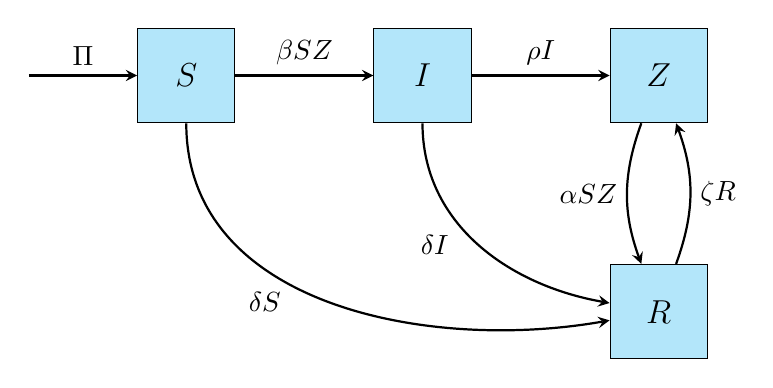
\begin{tikzpicture}[node distance=3cm]
	\node (S) [letter] {$S$};
	\node (I) [letter, right of=S] {$I$};
	\node (Z) [letter, right of=I, yshift=-0cm] {$Z$};
	\node (R) [letter, below of=Z, xshift=0cm, yshift=-0cm] {$R$};
	\draw [arrow] (S) -- node[anchor=south, xshift=0cm] {$\beta SZ$} (I);
	\draw [arrow] (I) -- node[anchor=south, xshift=0cm] {$\rho I$} (Z);
	\draw [arrow] (Z) to[out=-110, in=110] node[anchor=east, xshift=-.0cm] {$\alpha SZ$} (R);
	\draw [arrow] (R) to[out=70, in=-70] node[anchor=west, xshift=.0cm] {$\zeta R$} (Z);
	\draw [arrow] (S) to[out=-90, in=190] node[anchor=east, xshift=-.5cm] {$\delta S$} (R);
	\draw[arrow] (I) to[out=-90, in=170] node[anchor=east, xshift=-.25cm] {$\delta I$} (R);
	\draw[arrow] (-2,0) -- node[anchor=south, xshift=-.0cm] {$\Pi$} (S);
	\end{tikzpicture}
	\caption{The SIZR model.}
\end{figure}
% ----

The 4-Class model is thus described mathematically by the following system of ODEs:
\[S' = \Pi - \beta SZ - \delta S\]
\[I' = \beta SZ - \rho I - \delta I\]
\[Z' = \beta SZ + \zeta R - \alpha SZ\]
\[R' = \delta S + \alpha SZ - \zeta R\]
Hence, there are six parameters that determine the model dynamics: 
\begin{itemize}
	\item $\delta$: background (non zombie related) death rate,
	\item $\zeta$: zombie resurrection rate,
	\item $\beta$: zombie transmission rate,
	\item $\alpha$: zombie destruction rate,
	\item $\Pi$: birth rate,
	\item $\rho$: latent infection rate.
\end{itemize}

We pick the following parameter values to simulate our `true' zombie apocalypse data: $\delta=0.0001$, $\zeta= 0.0001$, $\beta=0.0095$, $\alpha=0.0005$, $\Pi=0.0001$, $\rho=0.05$. To solve the system of ODEs, we use Euler's method with a step size of 0.05. Figure \ref{true_epidemic} shows the dynamics using our chosen parameters. We treat this realisation of the model outbreak as our `observed' data, for which we will attempt to estimate the posterior of the parameters of our model using Approximate Bayesian Computation (ABC), which we will explain in detail in the following section.

\begin{figure}[H]
	\centering
	\includegraphics[width=0.8\linewidth]{../Figures/true_epidemic}
	\caption{`True' zombie apocalypse (`observed' data) simulated from model with chosen parameters (see main text).}
	\label{true_epidemic}
\end{figure}

\section{Approximate Bayesian Computation}

Likelihood-free inference methods are convenient for complex models, such as Epidemic models, where we do not have an explicit expression for the likelihood. In approximate Bayesian computation (ABC), simulation under the implicit model replaces computation of the likelihood. One can use simulations from the model for different parameter values to compare the simulated datasets with the observed data. These simulations are increasingly being used as training datasets for machine learning methods including deep neural networks \citep{RN6} and random forests \citep{RN8}. 

The use of ABC first became popular in the field of population genetics, where simulation from a range of models is possible, but the likelihood is intractable for realistic sized datasets. \cite{RN57} were the first to use ABC, conducting inference on human demographic history. The method has now been applied in various subject areas including systems biology \citep{RN60}, climate modelling \citep{RN61}, astronomy \citep{RN62} and epidemiology \citep{RN10}.

The goal of ABC is to find a posterior distribution for the parameters of the implicit model, explaining the complex and potentially high-dimensional dataset. The method is based on Bayesian statistics: updating our prior beliefs about the model parameters, where $\pi(\theta)$ is the prior, using the information from our simulations. Suppose the dataset consists of $n$ observations $y_{obs} = (y_{obs,1}, ..., y_{obs,n})$. A typical ABC procedure would involve mapping the observations to a lower dimensional set of summary statistics, $s(y)$. The posterior is then proportional to the following elements
\begin{equation}
p_{\epsilon}(\theta, s|s_{obs}) \propto \pi(\theta)f_n(s|\theta)K_{\epsilon}(\|s - s_{obs}\|),
\end{equation}
where $f_n(s|\theta)$ is the implicit density of the model, $K_{\epsilon}(x)$ is a kernel function with tolerance $\epsilon$, and $\| \cdot \|$ is a distance metric \citep{RN2}. The kernel function enables us to include in our posterior density the parameter values that best approximate the observations. This idea of estimating the likelihood of parameters using simulations that are `close' to the observed data dates back at least as far as \cite{RN56}.

As the tolerance value $\epsilon$ tends to zero, the simulations we accept are closer to the true data and the approximate posterior becomes closer to its true distribution. Unfortunately, in order to simulate the same number of points at a smaller tolerance level often requires many more simulations, and the simplest algorithms can quickly become computationally inefficient. Luckily, we can harness techniques such as Markov chain Monte Carlo \citep{RN17, RN27} and sequential Monte Carlo \citep{RN21, RN30, RN22, RN29} to improve the computational efficiency of ABC.

\subsection{Rejection algorithm}
\label{sec1}

Instead of pre-defining the tolerance level $\epsilon$, it is sometimes beneficial to simulate a set number of datasets $n$, of which we retain the proportion $p$ closest to the observed data. This version of the rejection algorithm is preferential in the scenario where one is unsure of a suitable tolerance to use a priori. The algorithm used in this report is outlined below:

\begin{algorithm}[H]
	\label{ABC Rejection} 
	\caption{ABC Rejection}
	\For{$i\leftarrow 1$ \KwTo $n$}{
		Sample $\theta_i \sim \pi(\theta)$\;
		Simulate data $y_i \sim f(y|\theta_i)$\;
		Transform data $y_i$ into summary statistics $s_i$ (optional)\;
		Calculate distance $\rho(s_i, s_{obs})$
	}
	Retain proportion $p$ with smallest distance
\end{algorithm}

\noindent Hence, in simple terms, the rejection algorithm consists of sampling parameters from a prior distribution and simulating datasets from a model using these parameters. One can then, optionally, transform these datasets into summary statistics, before retaining the proportion $p$ closest to the observations. The accepted sample of parameters then approximates the posterior distribution.

\subsection{Application to Zombie model}

In our case, the data $y_i$ is simulated from our model described in Section \ref{model} using Euler's method with a step size of 0.05. The summary statistics $s_i$ used in the rejection ABC algorithm are then simply daily values of susceptible individuals and zombies. Since we run the dynamics over a period of 25 days, this means we have a total of 50 summary statistics. Our `observed' data is the model dynamics simulated using the parameters stated in Section \ref{model} and illustrated in Figure \ref{true_epidemic}.

We run the ABC rejection algorithm with uniform priors on each of the parameters (over a reasonable range), $n=10,000$ simulations and retain the proportion $p=0.005$ closest to the observed data. Hence, we retain 50 parameter sets to build our approximate posterior distributions, as illustrated by the histograms in Figure \ref{rej_abc_posteriors}. We see that the posteriors for $\delta$, $\zeta$ and $\Pi$ do not vary greatly from the uniform priors, and the posterior means are quite far from the true parameters. The posteriors for $\beta$ and $\rho$ are slightly more interesting, and the posterior means seem to be closer to the true parameters; however, the posterior distributions do not concentrate well around the true parameters. Finally, for the parameter $\alpha$, the posterior mean almost exactly coincides with the true parameter; however, again the distribution does not concentrate well around this value and does not seem too different from the uniform prior.

In order to compare the rejection ABC algorithm to ABC with SMC in the following section, we report the maximal (normalised) distance (tolerance level) $\epsilon$ from the accepted summary statistics to the observed data: we get a value of $\epsilon = 26.56$. Using the \texttt{ABC\_rejection} function from the \texttt{EasyABC} R package, the algorithm took 13.30 seconds to run. 

To illustrate how close our accepted simulations are to the observed data, Figure \ref{rej_abc_acc_simulations} show a selection of 25 of the accepted simulations, alongside the observed dynamics. We can see that they vary quite greatly from the true data, indicating that the rejection ABC algorithms requires very large numbers of simulations in order to find the target parameter space. One can imagine that for a more expensive model to simulate from, this method would be too computationally expensive to be of any use.


\begin{figure}[H]
	\centering
	\includegraphics[width=1\linewidth]{../Figures/rejection_posteriors}
	\caption{The posterior distributions of the model parameters, attained from the ABC rejection algorithm, with $n=10,000$, $p=0.005$. The values of the true parameters are indicated by the red lines, while the posterior means are indicated by the green lines.}
	\label{rej_abc_posteriors}
\end{figure}

\begin{figure}[H]
\centering
\includegraphics[width=0.8\linewidth]{../Figures/rej_ABC_simulations}
\caption{The above figure shows a selection of simulations from the model with accepted parameter values from the ABC rejection algorithm, with $n=10,000$, $p=0.005$, alongside the `observed' dynamics.}
\label{rej_abc_acc_simulations}
\end{figure}

\begin{figure}[H]
	\centering
	\includegraphics[width=0.8\linewidth]{../Figures/rej_abc_sd_bands}
	\caption{The above figure compares the `observed' dynamics (solid curves) with the mean of the accepted simulations from the ABC rejection algorithm (dashed curves). The shaded regions indicate $\pm$ 1 standard deviation from the mean.}
	\label{rej_abc_sd}
\end{figure}




\section{Sequential Monte Carlo}

Sequential Monte Carlo (SMC) methods applied to ABC are concerned with reducing the number of model runs in order to achieve a certain quality of posterior approximation. We have now seen that the simple ABC rejection algorithm is very computationally demanding, which often limits applications to simple models; the number of simulations required to sample the entire parameter space grows exponentially with the number of parameters \citep{RN32}. SMC methods aim to progressively approximate the posterior using a decreasing sequence of tolerance levels $\{\epsilon_1, ..., \epsilon_T\}$. The idea is to sample from areas of the parameter space with a higher likelihood, rather than systematically from the whole space, in order to gain computational efficiency.

The basis of SMC algorithms is to construct a sequence of target distributions, that one propagates a set of particles through in order to move from the initial distribution to the final distribution. 

\subsection{Population Monte Carlo}

The first stage of the PMC ABC method of \cite{RN21} is identical to that of rejection ABC in Algorithm \ref{ABC Rejection}, giving the first stage approximation to the posterior distribution. One then resamples parameter values from a density kernel 
$$ q(\theta) = \sum_{j=1}^{N} w_j^{(t-1)} K(\theta| \theta_{j}^{(t-1)};\tau_t^2),$$ 
with $N$ being the number of samples in the first, and subsequent, iterations. A popular choice is a Gaussian kernel and \cite{RN21} shows that a good choice of $\tau$ is twice the empirical variance of the simulated parameters in the previous iteration. The bias that is induced by sampling from a proposal distribution, rather than the prior, is fixed by assigning an importance weight to each particle, as outlined in Algorithm \ref{PMC ABC} below. 


\begin{algorithm}[H]
	\label{PMC ABC}
	\caption{Population Monte Carlo ABC (PMC)}
	Given a decreasing sequence of tolerance levels $\{\epsilon_1, ..., \epsilon_T\}$\;
	\For{$t=1$}{
		\For{$i=1$ to $N$}{
			\textbf{until} $\rho(y, y_{obs}) < \epsilon_1$\;
			Simulate $\theta_{i}^{(1)} \sim \pi(\theta)$ and $y \sim f(y|\theta_{i}^{(1)})$ }
		Set $w_{i}^{(1)} = 1/N$ }
	\For{$t=2$ to $T$}{
		\For{$i=1$ to $N$}{
			\textbf{until} $\rho(y, y_{obs}) < \epsilon_t$\;
			Sample $\theta_{i}^{*}$ from $\theta^{(t-1)}_j$ with probabilities $w_j^{(t-1)}$\;
			Generate $\theta_{i}^{(t)} \sim K(\theta| \theta_{i}^{*};\tau_t^2)$ and $y \sim f(y|\theta_{i}^{(t)})$ }
		Set $w_{i}^{(t)} \propto \pi(\theta_{i}^{(t)}) / \sum_{j=1}^{N} w_j^{(t-1)} K(\theta_{i}^{(t)}| \theta_j^{(t-1)}; \tau_t^2)$\;
		Set $\tau_{t+1}^2$ as twice the weighted emprirical variance of the $\theta_i^{(t)}$'s}
\end{algorithm}	

A drawback of this method is that it requires the user to pre-define a decreasing sequence of tolerance levels $\{\epsilon_1, ..., \epsilon_T\}$. A poor choice of sequence could detriment the possible benefits of the importance sampling procedure. In the population genetic example conducted by \cite{RN21}, $\epsilon_1$ is based on a preliminary simulation as the 0.1 quantile and they perform four iterations with $\epsilon_2 = 0.75\epsilon_1$, $\epsilon_3 = 0.9\epsilon_2$ and $\epsilon_4 = 0.9\epsilon_3$.

\subsection{Application to Zombie model}


sequence of tolerance levels: $\{ 10, 5, 1, 0.5\}$

no of simulations performed: 4096

Compute time: 2.89 seconds

max epsilon of accepted simulations: 0.489

\begin{figure}[H]
	\centering
	\includegraphics[width=0.8\linewidth]{../Figures/PMC-ABC_simulations}
	\caption{The above figure shows a selection of simulations from the model with accepted parameter values from the PMC-ABC algorithm, with the decreasing sequence of tolerance levels $\{ 10, 5, 1, 0.5\}$ and $N=50$, alongside the `observed' dynamics.}
	\label{pmc_abc_acc_simulations}
\end{figure}

\begin{figure}[H]
	\centering
	\includegraphics[width=0.8\linewidth]{../Figures/PMC_ABC_sd_bands}
	\caption{The above figure compares the `observed' dynamics (solid curves) with the mean of the accepted simulations from the PMC-ABC algorithm (dashed curves). The shaded regions indicate $\pm$ 1 standard deviation from the mean.}
	\label{pmc_abc_sd}
\end{figure}

\begin{figure}[H]
	\centering
	\includegraphics[width=1\linewidth]{../Figures/PMC_posteriors}
	\caption{The posterior distributions of the model parameters, attained from the PMC-ABC algorithm, with the decreasing sequence of tolerance levels $\{ 10, 5, 1, 0.5\}$ and $N=50$. The values of the true parameters are indicated by the red lines, while the posterior means are indicated by the green lines.}
	\label{pmc_abc_posteriors}
\end{figure}


\bibliography{references}
\end{document}
